\documentclass[format=sigconf]{acmart}
\acmConference[ICONS 2020]{International Conference on Neuromorphic Systems}{July 2020}{Chicago, Illinois}
\keywords{deep learning, neural network, biologically-motivated, equilibrium propagation, vanishing gradient, small-world, neuromorphic hardware}

%\usepackage{cite}
\usepackage{natbib}
\usepackage{graphicx}
\usepackage{bm}
\usepackage{amsmath}
%\usepackage{amssymb}
\usepackage{subcaption}
\usepackage{mathtools}
\usepackage[title]{appendix}
\usepackage[ruled,vlined]{algorithm2e}
\usepackage{hyperref}
\usepackage{adjustbox}
\usepackage[title]{appendix}

\newcommand{\mtx}[1]{\bm{#1}}
\newcommand{\rms}[1]{<{#1}>}
\newcommand{\npar}{\\\indent}
\DeclareMathOperator*{\minimize}{minimize}

\title{Layer-skipping connections facilitate training of layered networks using equilibrium propagation.}
\author{Jimmy Gammell}
\author{Sae Woo Nam}
\author{Adam N. McCaughan}

\begin{CCSXML}
<ccs2012>
   <concept>
       <concept_id>10010147.10010257.10010293.10011809</concept_id>
       <concept_desc>Computing methodologies~Bio-inspired approaches</concept_desc>
       <concept_significance>500</concept_significance>
       </concept>
   <concept>
       <concept_id>10010147.10010257.10010293.10010294</concept_id>
       <concept_desc>Computing methodologies~Neural networks</concept_desc>
       <concept_significance>500</concept_significance>
       </concept>
%   <concept>
%       <concept_id>10010147.10010257.10010258.10010259</concept_id>
%       <concept_desc>Computing methodologies~Supervised learning</concept_desc>
%       <concept_significance>300</concept_significance>
%       </concept>
 </ccs2012>
\end{CCSXML}

\ccsdesc[500]{Computing methodologies~Bio-inspired approaches}
\ccsdesc[500]{Computing methodologies~Neural networks}
%\ccsdesc[300]{Computing methodologies~Supervised learning}

\begin{document}

\begin{abstract}

Equilibrium propagation is a learning framework for energy-based networks that can be implemented by neurons that perform only one type of computation in the prediction and correction phases of training, and that computes parameter corrections for a given neuron using only the activation values of directly-connected neurons. This makes it an appealing candidate for implementation in neuromorphic analog hardware, and marks a step forward in the search for a biologically-plausible implementation of deep learning. However, in previous implementations of equilibrium propagation, layered networks suffered from a vanishing gradient problem that has not yet been solved in a simple, biologically-plausible way. In this paper, we demonstrate that the vanishing gradient problem can be counteracted by replacing some of a layered network's connections with random layer-skipping connections in a manner inspired by small-world networks. This approach could be conveniently implemented in neuromorphic analog hardware and is biologically-plausible.

\end{abstract}

\maketitle

\section{Introduction}

The equilibrium propagation learning framework \cite{scellier17} is a method for training a class of energy-based networks, the prototype for which is the continuous Hopfield network \cite{hopfield1984}. It is appealing because it addresses some major issues that prevent backpropagation from being biologically-plausible, and as a side-effect could be implemented in neuromorphic analog hardware more-easily than backpropagation.
\npar
A major reason backpropagation is not biologically-plausible is that to implement it in a system lacking an omniscient supervisor (i.e. code that can easily access all parameters and activations in the network), each neuron would require one mechanism by which to pass its activation to shallower neurons during the forward-propagation phase and a second mechanism by which to pass deeper neurons the necessary information to correct their parameters during the backpropagation phase (including precise information about the manner in which their activations are propagated to the network's output) \cite{bengio2015}. In contrast, equilibrium propagation allows a neuron to compute corrections to its parameters using only the activations of neighboring neurons, allowing both the prediction and correction phases of training to be carried out using a single information-transfer mechanism \cite{scellier17}.
\npar
Another issue with backpropagation is that neurons are required to perform distinct operations during the forward and backward propagation phases - in the forward propagation phase they pass forward an activation value that is a function of the activations of deeper neurons, whereas in the backward propagation phase they pass backwards an error term that is a different function of error terms from shallower neurons. This implies two distinct sets of computational circuitry in each neuron. In equilibrium propagation the only difference between the prediction and correction phases of training is that in the correction phase output neurons are weakly-clamped towards the target output; the dynamics by which the network evolves are otherwise the same \cite{scellier17}.
\npar
Because of these differences, relative to backpropagation, equilibrium propagation could be implemented more-easily in neuromorphic analog hardware, and it is more-plausible that it could be carried out by observed architecture in biological brains.
\npar
It has been demonstrated \cite{scellier17} that a continuous Hopfield network with a basic layered topology can be trained on MNIST \cite{mnist1998} through the equilibrium propagation framework. However, previous implementations encountered a vanishing gradient problem (section \ref{sec:vangrad}) that significantly impedes training of networks with several hidden layers. Given that network depth is critical for performance on difficult datasets \cite{simonyan2014, srivastava2015tvdn}, and that convergence to a low error rate on MNIST is a low bar for a network to meet, this is a nontrivial issue. It has been demonstrated \cite{scellier17} that the problem can be solved by using a unique learning rate for parameters at different depths in the network, with deeper parameters trained with larger learning rates to counteract gradient attenuation with depth. This approach is unappealing because (1) it introduces additional hyperparameters that must be tuned, (2) it would be inconvenient to implement and tune unique learning rates in analog hardware, and (3) it has not been observed in biological systems.
\npar
The purpose of this paper is to introduce a modification to the layered topology that can counteract the vanishing gradient problem in the context of energy-based networks trained using equilibrium propagation. The modification is inspired by small-world topology \cite{watts98}, and consists of first fully-connecting a network's layers, then replacing some of its connections with random layer-skipping connections. We achieve 0\% training error (out of 50,000 examples) and under 2.5\% test error (out of 10,000 examples) on MNIST using a network with 3 hidden layers and no regularization term in its cost function. These error rates are comparable to those achieved by other biologically-motivated networks \cite{bartunov2018} and are the same as those achieved in the original paper using a layered topology and manually-tuned per-layer learning rates \cite{scellier17}, albeit they are achieved after around 25\% more epochs. Our method adds only one additional hyperparameter - the number of connections to randomly replace - while removing $L-2$ parameters, where $L$ is the number of layers in the network. It could be implemented with relative ease in any system with configurable connectivity.
\footnote{Our current implementation also requires manual tuning of the initial weights of intralayer and layer-skipping connections, but we have found that networks are not very sensitive to these initializations and that performance is good as long as they are in the same ballpark as the rest of the network's initializations.} Layer-skipping connections have been observed in biological brains \cite{bullmore2009}, so this approach is biologically-plausible. Similar techniques have been used with some success to modify convolutional \cite{he2015, srivastava2015} and multilayer feedforward \cite{xiaohu2011, krishnan2019} networks with varying degrees of success. Our findings in this paper show that layer-skipping connections are effective enough to be appealing in contexts where simplicity and biological plausibility are important.


\section{Background and Theory}

\subsection{Equilibrium propagation}
\label{sec:eqp_formulation}

Equilibrium propagation \cite{scellier17} is a learning framework for energy-based networks that trains their parameters by approximating gradient descent on some arbitrary cost function. It is applicable to any network with dynamics characterized by evolution to a fixed point of an associated energy function; in this and in \cite{scellier17}, it is implemented on a continuous Hopfield network \cite{hopfield1984}. For a variety of reasons outlined in \cite{bengio2015}, backpropagation is not biologically-plausible. One of the major reasons is that to correct the parameters of a given neuron, backpropagation requires precise information about the activations and nonlinearities of all neurons in the corresponding feedforward path; equilibrium propagation avoids this problem by correcting a neuron's parameters using only the activations of neurons to which it directly connects. Another major reason backpropagation is not biologically-plausible is that it requires neurons to perform distinct computations (implemented using distinct circuitry) in the forward and backward propagation phases of training; in contrast, equilibrium propagation requires only one behavior of neurons in both the prediction (free) and correction (weakly-clamped) phases of training. In addition to enhancing its biological plausibility, these traits make equilibrium propagation appealing as a framework to implement on neuromorphic analog hardware because they would limit the complexity required of neurons and the amount of infrastructure needed to operate and train them.

\subsubsection{Implementation in a continuous Hopfield network}

Here we summarize the equations through which a continuous Hopfield network is trained using equilibrium propagation; this summary is based on the more-thorough and more-general treatment in \cite{scellier17}.
\npar
Consider a network with $n$ neurons organized into an input layer with $p$ neurons, hidden layers with $q$ neurons and an output layer with $r$ neurons. Let the activations of these neurons be denoted by vectors $\mtx{x}\in\mathbb{R}^{p}$, $\mtx{y}\in\mathbb{R}^{q}$ and $\mtx{h}\in\mathbb{R}^{r}$, and let $\mtx{s}=(\mtx{h}^{T},\mtx{y}^{T})^{T}\in\mathbb{R}^{q+r}$ and $\mtx{u}=(\mtx{x}^{T}, \mtx{s}^{T})^{T}\in\mathbb{R}^{n}$ be vectors of, respectively, the activations of non-fixed (non-input) neurons and of all neurons in the network. Let $\mtx{W}\in\mathbb{R}^{n\times n}$ and $\mtx{b}\in\mathbb{R}^{n}$ denote the network's weights and biases where $w_{ij}$ is the connection weight between neurons $i$ and $j$ and $b_i$ is the bias for neuron $i$ ($\forall i \;w_{ii}=0$ to prevent self-connections), and let $\rho$ denote its activation function; here and in \cite{scellier17},
\begin{equation}
\label{eqn:hardened_sigmoid}
\rho(x)=\begin{cases}0&x<0\\x&0\leq x\leq 1\\1&x>1\end{cases} 
\end{equation} \sloppy is a hardened sigmoid function
where $\rho'(0)=\rho'(1)$ is defined to be 1 to avoid neuron saturation. Let $\mtx{\rho}((x_1,\hdots, x_n)^T)=(\rho(x_1),\hdots,\rho(x_n))^T$.
\npar
The behavior of the network is to perform gradient descent on a total energy function $F$ that is modified by a training example $(\mtx{x}_d,\mtx{y}_d)$. Consider energy function $E:\mathbb{R}^n\to\mathbb{R}$,
\begin{equation}
E(\mtx{u}; \mtx{W}, \mtx{b})=\frac{1}{2}\mtx{u}^T\mtx{u}-\frac{1}{2}\mtx{\rho}(\mtx{u})^T \mtx{W} \mtx{\rho}(\mtx{u})-\mtx{b}^T\mtx{u}
\end{equation}
and arbitrary cost function $C:\mathbb{R}^r\to\mathbb{R}_{+}$; here and in \cite{scellier17} it is a quadratic cost function given by
\begin{equation}
\label{eqn:cost}
C(\mtx{y})=\frac{1}{2}||\mtx{y}-\mtx{y}_d||_2^2,
\end{equation}
though the framework still works for cost functions incorporating a regularization term dependent on $\mtx{W}$ and $\mtx{b}$. The total energy function $F:\mathbb{R}^n\to\mathbb{R}$ is given by
\begin{equation}
F(\mtx{u}; \beta, \mtx{W}, \mtx{b})=E(\mtx{u};\mtx{W}, \mtx{b})+\beta C(\mtx{y})
\end{equation}
where the clamping factor $\beta$ is a small constant. $\mtx{s}$ evolves over time $t$ as
\begin{equation}
\label{eqn:dynamics}
\frac{d\mtx{s}}{dt}\propto -\frac{\partial F}{\partial \mtx{s}}.
\end{equation}
Equilibrium has been reached when $\frac{\partial F}{\partial \mtx{s}} \approx 0$. This can be viewed as solving the optimization problem
\begin{equation}
	\minimize_{\mtx{s}\in\mathbb{R}^{q+r}}F((\mtx{x}_d^T,\mtx{s}^T)^T; \beta, \mtx{W}, \mtx{b}) 
\end{equation}
by using gradient descent to find a local minimum of $F$.
\npar
The procedure for training on a single input-output pair $(\mtx{x}_d,\mtx{y}_d)$ is as follows:
\begin{enumerate}
\item Clamp $\mtx{x}$ to $\mtx{x}_d$ and perform the free-phase evolution: evolve to equilibrium on the energy function $F(\mtx{u}; 0, \mtx{W}, \mtx{b})$ in a manner dictated by equation \ref{eqn:dynamics}. Record the equilibrium state $\mtx{u}^0$.
\item Perform the weakly-clamped evolution: evolve to equilibrium on the energy function $F(\mtx{u}; \beta, \mtx{W}, \mtx{b})$ using $\mtx{u}^0$ as a starting point. Record the equilibrium state $\mtx{u}^{\beta}$.
\item Compute the correction to each weight in the network: 
\begin{equation}
\label{eqn:weight_correction}
\Delta W_{ij}=\frac{1}{\beta}(\rho(u_i^\beta)\rho(u_j^\beta)-\rho(u_i^0)\rho(u_j^0)).
\end{equation}
Adjust the weights using $W_{ij}\leftarrow W_{ij}+\alpha\Delta W_{ij}$ where the learning rate $\alpha$ is a positive constant.
\item Compute the correction to each bias in the network:
\begin{equation}
\Delta b_i=\frac{1}{\beta}(\rho(u_i^{\beta})-\rho(u_i^0))
\end{equation}
and adjust the biases using $b_i\leftarrow b_i+\alpha\Delta b_i$.
\end{enumerate}
This can be repeated on as many training examples as desired. Training can be done on batches by computing $\Delta W_{ij}$ and $\Delta b_i$ for each input-output pair in the batch, and correcting using the averages of these values. Note that the correction to a weight is computed using only the activations of neurons it directly affects, and the correction to a bias is computed using only the activation of the neuron it directly affects. This contrasts with backpropagation, where to correct a weight or bias $l$ layers from the output it is necessary to know the activations, derivatives and weights of all neurons between $0$ and $l-1$ layers from the output.

\subsubsection{Approximation of equation of motion}

In analog hardware the dynamics described by equation \ref{eqn:dynamics} could be implemented efficiently using leaky integrator neurons, but on digital hardware it is necessary to discretize and approximate these dynamics; we now describe the approximation used here and in \cite{scellier17}. Let $\mtx{s}[n]$ denote the state of the network after $n$ iterations of the approximation, $N$ denote the total number of iterations and $\epsilon$ the size of each iteration. $\mtx{s}[0]$ is the initial state of the network; here and in \cite{scellier17}, $\mtx{s}[0]=\mtx{0}$ before the first epoch, and in subsequent epochs $\mtx{s}[0]$ is the equilibrium state of the network from the last time it executed a free phase on the same batch. Let 
 \begin{equation}
 s_i[n]=s_i[n-1]-\epsilon \frac{\partial F}{\partial s_i},\;n=1,\hdots,N
 \end{equation}
(where $\beta=0$ in the free phase); then $\mtx{s}[N]$ approximates the state after time $\epsilon N$ that would be given by equation \ref{eqn:dynamics}.
 We denote the number of iterations in the free and weakly-clamped phases $N_{free}$ and $N_{weakly-clamped}$, respectively. It is only necessary to run the weakly-clamped phase long enough to observe the initial direction in which the network evolves and to allow the perturbation of the output to influence all layers in the network, so typically for a network with $L$ layers, $N_{free}>>N_{weakly-clamped}>L$.

\subsection{Vanishing gradient problem}
\label{sec:vangrad}

It has been observed \cite{scellier17} that energy-based networks with a layered topology trained using equilibrium propagation suffer from a vanishing gradient problem whereby the rate of training of a weight decreases approximately exponentially with the number of layers between that weight and the output layer. This is problematic because it has been observed to increase the time needed to train a network, and gradients spanning several orders of magnitude could be hard to represent in analog implementations of the framework with limited bit depth. The vanishing gradient problem is familiar in the context of conventional networks trained through backpropagation, where the composition of many layers can impede training by amplifying or attenuating the effect of changes to deep neurons as these changes propagate to the output layer, leading to a vanishing or exploding gradient. For those networks the problem can be effectively addressed by initializing weights to make activation variances and backpropagated gradient variances approximately uniform with respect to depth as described in \cite{glorot2010}, and by using activation functions with derivatives that do not cause neurons to saturate \cite{schmidhuber2015}, such as rectified linear units $\rho(x)=\text{Max}\{0, x\}$ or hardened sigmoids (equation \ref{eqn:hardened_sigmoid}). Batch normalization \cite{ioffe2015} is another effective technique for promoting uniform training in a network; inputs to each layer are whitened (the input distribution $\bf{X}$ to each layer is transformed to have $E[\bf{X}]=0$ and $Var[\bf{X}]=1$) during each batch to prevent changes to deep parameters from changing the input distribution to shallower layers and requiring adjustment to compensate.
\npar
The weight initialization scheme from \cite{glorot2010} and the use of hardened sigmoid activation functions do not solve the vanishing gradient problem in the context of equilibrium propagation. Batch normalization has not been tried in this context, but is not biologically-plausible. This suggests that the cause of the vanishing gradient problem here is different than in a conventional network. The situation in energy-based networks is more-complicated because there is no straightforward relationship between the activations of two given neurons; instead, neurons evolve as a coupled dynamical system.
\npar
In \cite{scellier17} the vanishing gradient problem was addressed by using unique learning rates for each layer, chosen to make the magnitudes of corrections to neurons' parameters uniform regardless of depth in the network. While this method is effective, it is unappealing because it seems unlikely to take place in a biological brain, it would add complexity to an analog implementation of the framework, and it introduces more hyperparameters that must be tuned to train a network. Our topology effectively addresses the problem without these unappealing characteristics.


\subsection{Small-world networks}
\label{sec:sw_background}

Our topology was inspired by small-world graph topology as described in \cite{watts98}. We have observed that energy-based networks with layered topology experience exponential attenuation of the gradient of a given parameter as its depth in the network increases, so it seems reasonable to expect that the vanishing gradient problem can be reduced by decreasing the number of connections needed to move between a given neuron and the output layer. Small-world topology offers a way to do this while largely preserving clustering between neurons within the same layer. It is also a topology that has been observed in biological brains \cite{bullmore2009}. Essentially, a layered network with fully-connected layers can be viewed as a network with a large typical path length between pairs of neurons and a large amount of clustering between nearby neurons. By randomly replacing a small proportion of its connections, its typical path length can be greatly reduced without significantly reducing its clustering. Quantitative metrics of a network's small-worldness are described in appendix \ref{app:sw_metrics}, but in our experiments these metrics have little correlation with network behavior (we discuss this further in section \ref{sec:disc_factors}).

\subsubsection{Algorithm for generating a small-world graph}
\label{sec:sw_algorithm}


\begin{algorithm}
\DontPrintSemicolon
\KwIn{A regimented graph $G$}
\KwIn{A probability $p$}
\tcp{Probability with which to replace a given preexisting edge}
\KwOut{Resulting modified graph}
\For{$\text{edge }e\in G$}
{
	$p'\sim U[0,1]$;\\
	\If{$p'\leq p$}
	{
		$\text{Add edge between random unconnected pair of vertices}$;\\
		$\text{Remove }e$;
	}
}
\Return{$G$}

\caption{Algorithm to generate small-world graph}
\label{alg:sw}
\end{algorithm}


Algorithm \ref{alg:sw} was introduced in \cite{watts98} to convert a regimented graph into a small-world graph. It was implemented on a lattice graph but works equally-well for the topology of a layered neural network. As $p\approx 0$ is increased, the mean shortest path between a pair of vertices in the graph ($L$ from appendix \ref{app:sw_metrics}) decreases rapidly while preexisting clusters remain largely intact ($C$ from appendix \ref{app:sw_metrics} does not significantly decrease). To generate a small-world graph, $p$ is chosen so that the graph has a large amount of clustering and a small mean shortest path, relative to a random graph with the same number of vertices and edges ($\sigma$ from appendix \ref{app:sw_metrics} is large).


\section{Implementation}

\begin{figure}
  \centering
    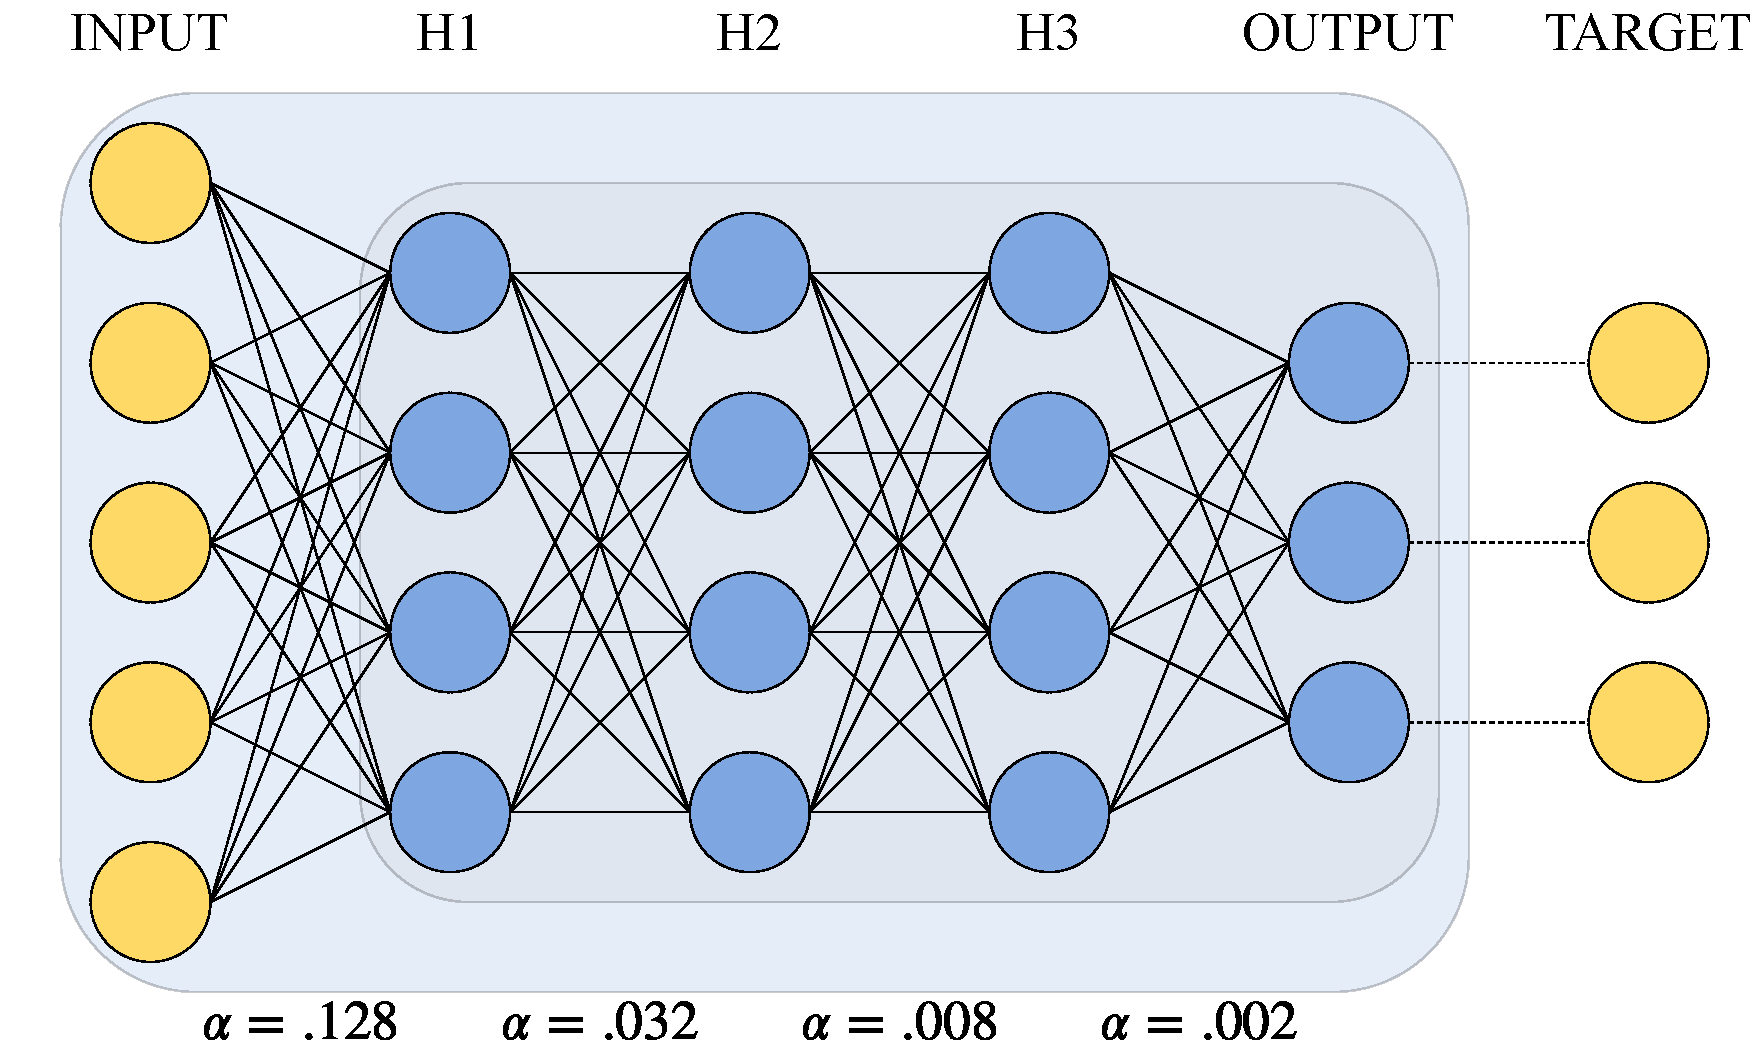
\includegraphics[width=\columnwidth]{figures/basic_topology_illustration.pdf}
    \caption{Topology of the layered network tested in \cite{scellier17}. All pairs of neurons in adjacent layers are connected, and there are no additional connections. All connections are bidirectional. The learning rate for weights is reduced by a factor of 4 each time distance from the output decreases by one layer, to compensate for the vanishing gradient problem.}
    \label{fig:top_basic}
\end{figure}
\hfill
\vspace{4mm}
\begin{figure}
	\centering
    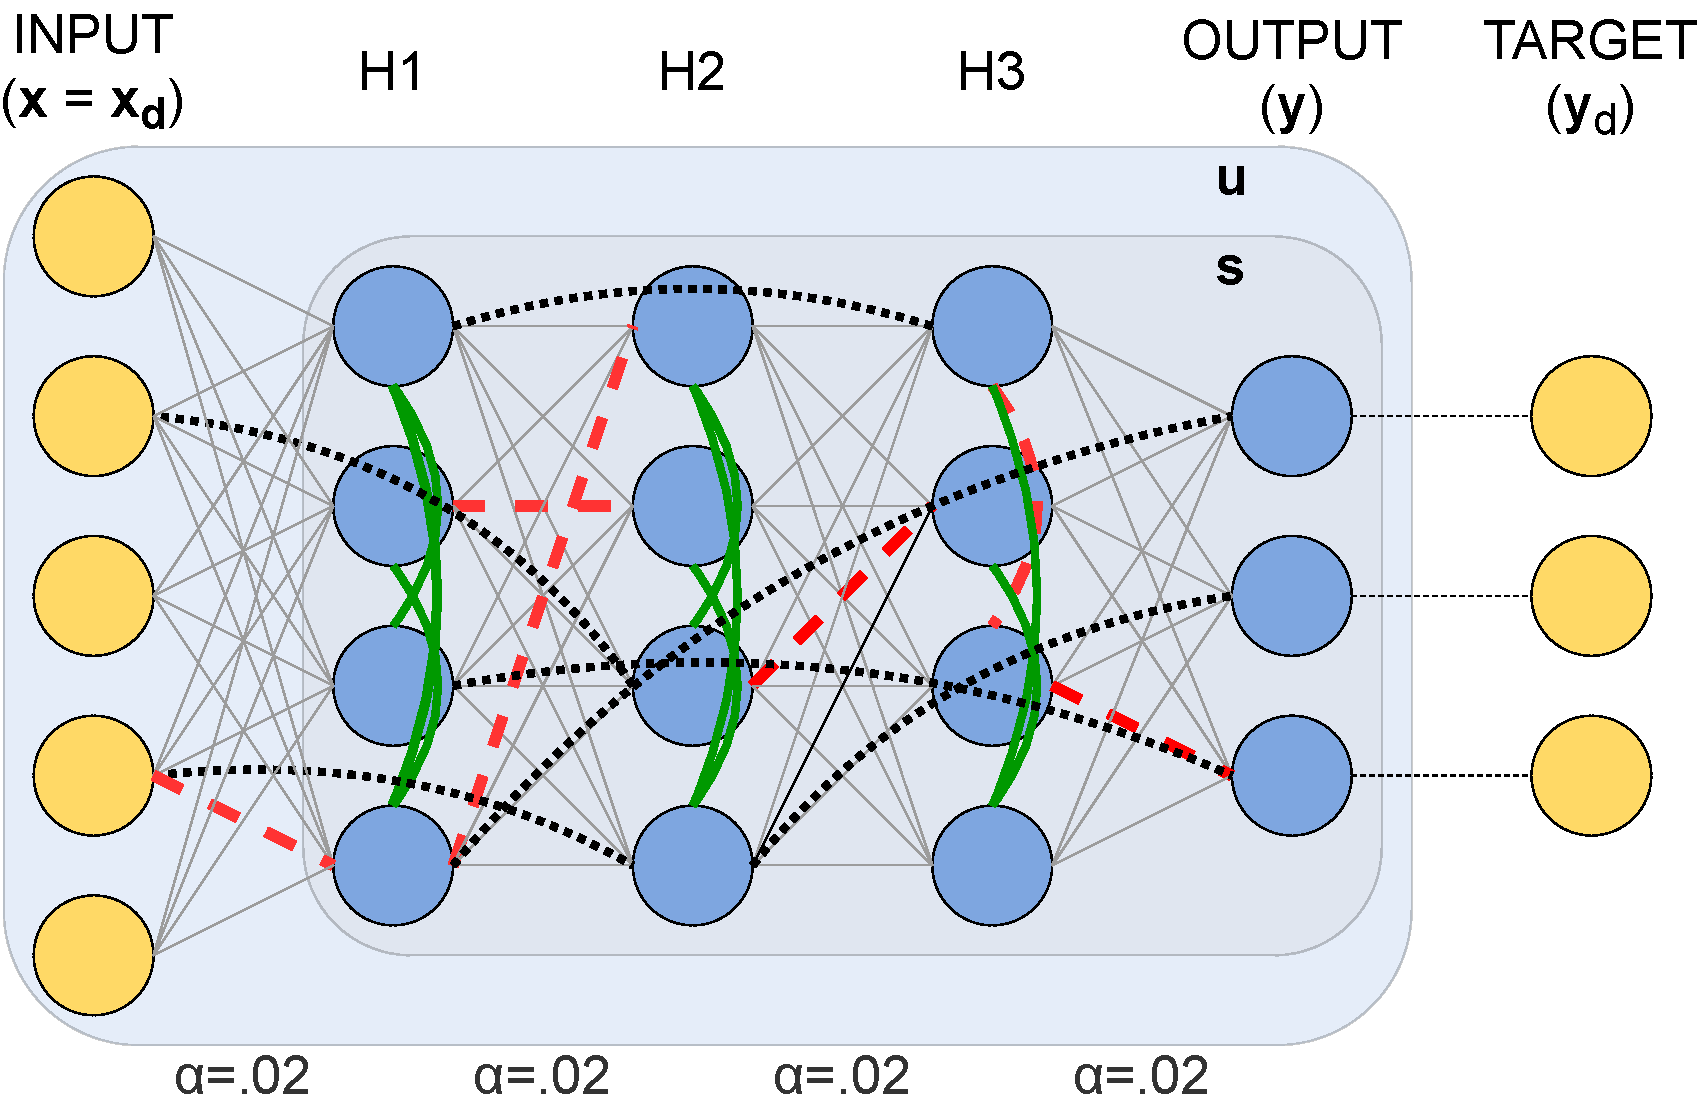
\includegraphics[width=\columnwidth]{figures/topology_changes_illustration.pdf}
     \caption{Changes to the layered topology to compensate for the vanishing gradient problem while using a single learning rate for all weights. Red dotted lines denote connections that have been removed and black dotted lines denote their replacements. Green solid lines denote added intralayer connections. In this illustration connections have been replaced by a random layer-skipping connection with probability $p\approx 8\%$. All connections are bidirectional.}

    \label{fig:top_sw}
\end{figure}

We implemented
\footnote{\url{https://github.com/jgammell/Equilibrium_Propagation_mobile.git}}
 the equilibrium propagation learning framework \cite{scellier17} using the Pytorch library, and verified that we could recreate the experiments ran in \cite{scellier17}. We follow the procedure described in section \ref{sec:eqp_formulation}; we use a hardened sigmoid activation function (equation \ref{eqn:hardened_sigmoid}) and a squared-error cost function with no regularization term (equation \ref{eqn:cost}). Testing was done on the MNIST dataset \cite{mnist1998} with input-output pairs grouped into batches of 20; training was done on the 50,000 training pairs and testing on the 10,000 validation pairs.
\npar
We use two performance-boosting techniques described in \cite{scellier17}. We randomize the sign of $\beta$ at the outset of each batch, which provides a regularization effect (note that parameter corrections are divided by $\beta$, so are changed to minimize cost regardless of its sign). We use persistent particles: after the first epoch, before training on a batch the network's state is initialized to its free equilibrium state from the last time it trained on the same batch. This reduces computational resources needed for training by reducing the number of iterations of equation \ref{eqn:dynamics} needed to reach equilibrium, and would be unnecessary in an analog implementation; note that training and test error rates during early epochs are artificially inflated as a result of this technique.

\subsection{Layered topology with unique learning rates}
\label{sec:basic_topology}

We recreated the 5-layer network used in \cite{scellier17}. It has a standard layered topology shown in \ref{fig:top_basic}.
\npar
The network consists of an input layer with 784 neurons, 3 hidden layers with 500 neurons each, and an output layer with 10 neurons. There are connections between every pair of neurons in adjacent layers, no connections between neurons in the same layer, and no layer-skipping connections.
\npar
The weight matrix was initialized using the Glorot-Bengio initialization scheme \cite{glorot2010}: a weight connecting layer $j$ with $n_j$ neurons to layer $j+1$ with $n_{j+1}$ neurons is drawn from a uniform distribution
\begin{equation}
\label{eqn:gb_init}
U[-\frac{\sqrt{6}}{\sqrt{n_j+n_{j+1}}},\frac{\sqrt{6}}{\sqrt{n_j+n_{j+1}}}].
\end{equation}
For effective training it is necessary to use unique learning rates to train the weights connecting each pair of layers. We use the same learning rates that were used for experiments in \cite{scellier17}: .128, .032, .008, .002, in order of the deepest to the shallowest layer; to counter the vanishing gradient problem the learning rate is reduced by a factor of 4 each time the distance from the output layer decreases by one layer. Each neuron has a bias term that is trained using the learning rate corresponding to the weights of the neuron's input connections, e.g. the biases of the first hidden layer are trained with a learning rate of .128.

\subsection{Layered topology with single learning rate}
\label{sec:basic_topology_uniform}

To provide a point of reference, we ran tests on a network that is identical to that in section \ref{sec:basic_topology} except with a single learning rate of .02 across the entire network. It performs poorly due to the vanishing gradient problem.

\subsection{Our topology}
\label{sec:our_topology}


\begin{algorithm}
\KwIn{A network $N$ with layered topology}
\tcp{described in section \ref{sec:basic_topology_uniform}}
\KwIn{An integer $n$}
\tcp{number of connections to replace}
\KwOut{A network with our modified topology}
\For{$\text{hidden layer }l\in N$}
{
	$\text{Add edge between each pair of neurons in }l$
}
\For{$i\leftarrow 1$ \KwTo $n$}
{
	$\text{Randomly select connection }c\in N$;\\
	$\text{Add connection between random unconnected pair of neurons}\in N$;\\
	\tcp{Do not allow self connections}
	\tcp{Do not allow connections between two input neurons or between two output neurons}
	$\text{Remove }c$;
}
\Return{$N$}

\caption{Algorithm to produce our topology}
\label{alg:ourtop}
\end{algorithm}

To generate a network with our topology, we use algorithm \ref{alg:ourtop}. The topology is illustrated in figure \ref{fig:top_sw}. For $p\lesssim .2$, algorithm \ref{alg:ourtop} is roughly equivalent to algorithm \ref{alg:sw} with $p=1-(\frac{N_o-1}{N_o})^n$, where $N_o$ is the number of connections in the network
\footnote{Algorithm \ref{alg:sw} with large $p$ produces more layer-skipping connections than algorithm \ref{alg:ourtop} with large $n$; it can be shown that for any $n$, algorithm \ref{alg:ourtop} is equivalent to algorithm \ref{alg:sw} with ${p=N_l-N_l\sqrt[N_o]{\frac{N_l}{N_o+N_l}+\frac{N_o}{N_o+N_l}(1-\frac{N_o+N_l}{N_oN_l})^n}}$ where $N_l$ is the number of unconnected pairs of neurons that are candidates to share a layer-skipping connection.}
; to contextualize the number of replaced connections, we will henceforth describe networks with our topology in terms of $p$ and not $n$. We have also tried adding new connections without removing existing ones, and observed roughly the same performance; in this paper we replace connections to limit the number of parameters added to the network. We do not add connections within the input or output layers and we do not allow neurons to connect to themselves. We have seen good results with $p\approx 8\%$.
\npar
This topology allows us to train the network with a uniform learning rate of .02 across the entire network. Weights of connections between pairs of neurons in adjacent layers are still initialized based on equation \ref{eqn:gb_init}. Weights of intralayer connections and layer-skipping connections are drawn from the uniform distribution $U[-.05,.05]$, where the value .05 was chosen empirically to optimize network performance.

\subsection{Tracking the training rates of individual pairs of layers}

We find it informative to track the root-mean-square magnitude of corrections to weights in individual layers; if $\Delta w_{ij}^l(b)$ denotes the correction to the connection weight between the $i^{th}$ neuron in layer $l$ and the $j^{th}$ neuron in layer $l+1$ in response to batch $b$ and $N^l$ denotes the number of neurons in layer $l$, we define
\begin{equation}
\label{eqn:rms_correction}
\Delta w^l(b):=\sqrt{\frac{\sum_{i=1}^{N^l}\sum_{j=1}^{N^{l+1}}(\Delta w_{ij}^l(b))^2}{N^lN^{l+1}}}
\end{equation}
as a metric of the extent to which the weights between layers $l$ and $l+1$ trained in response to batch $b$. We ignore the training of the weights of intralayer and layer-skipping connections.
\npar
This measurement is volatile, so for clarity we plot the average of $\Delta w^l(b')$ for $b'$ in a neighborhood of batch $b$: for some $n$, we define
\begin{equation}
\label{eqn:running_avg}
\Delta \hat{w}^l(b):=\frac{1}{2n+1}\sum_{b'=b-n}^{b+n}\Delta w^l(b').
\end{equation}
Comparing the traces $\Delta \hat{w}^l(b)$ vs. $b$ for different layers reveals the extent of the vanishing gradient problem.

\section{Results}

\begin{figure}
  \centering
  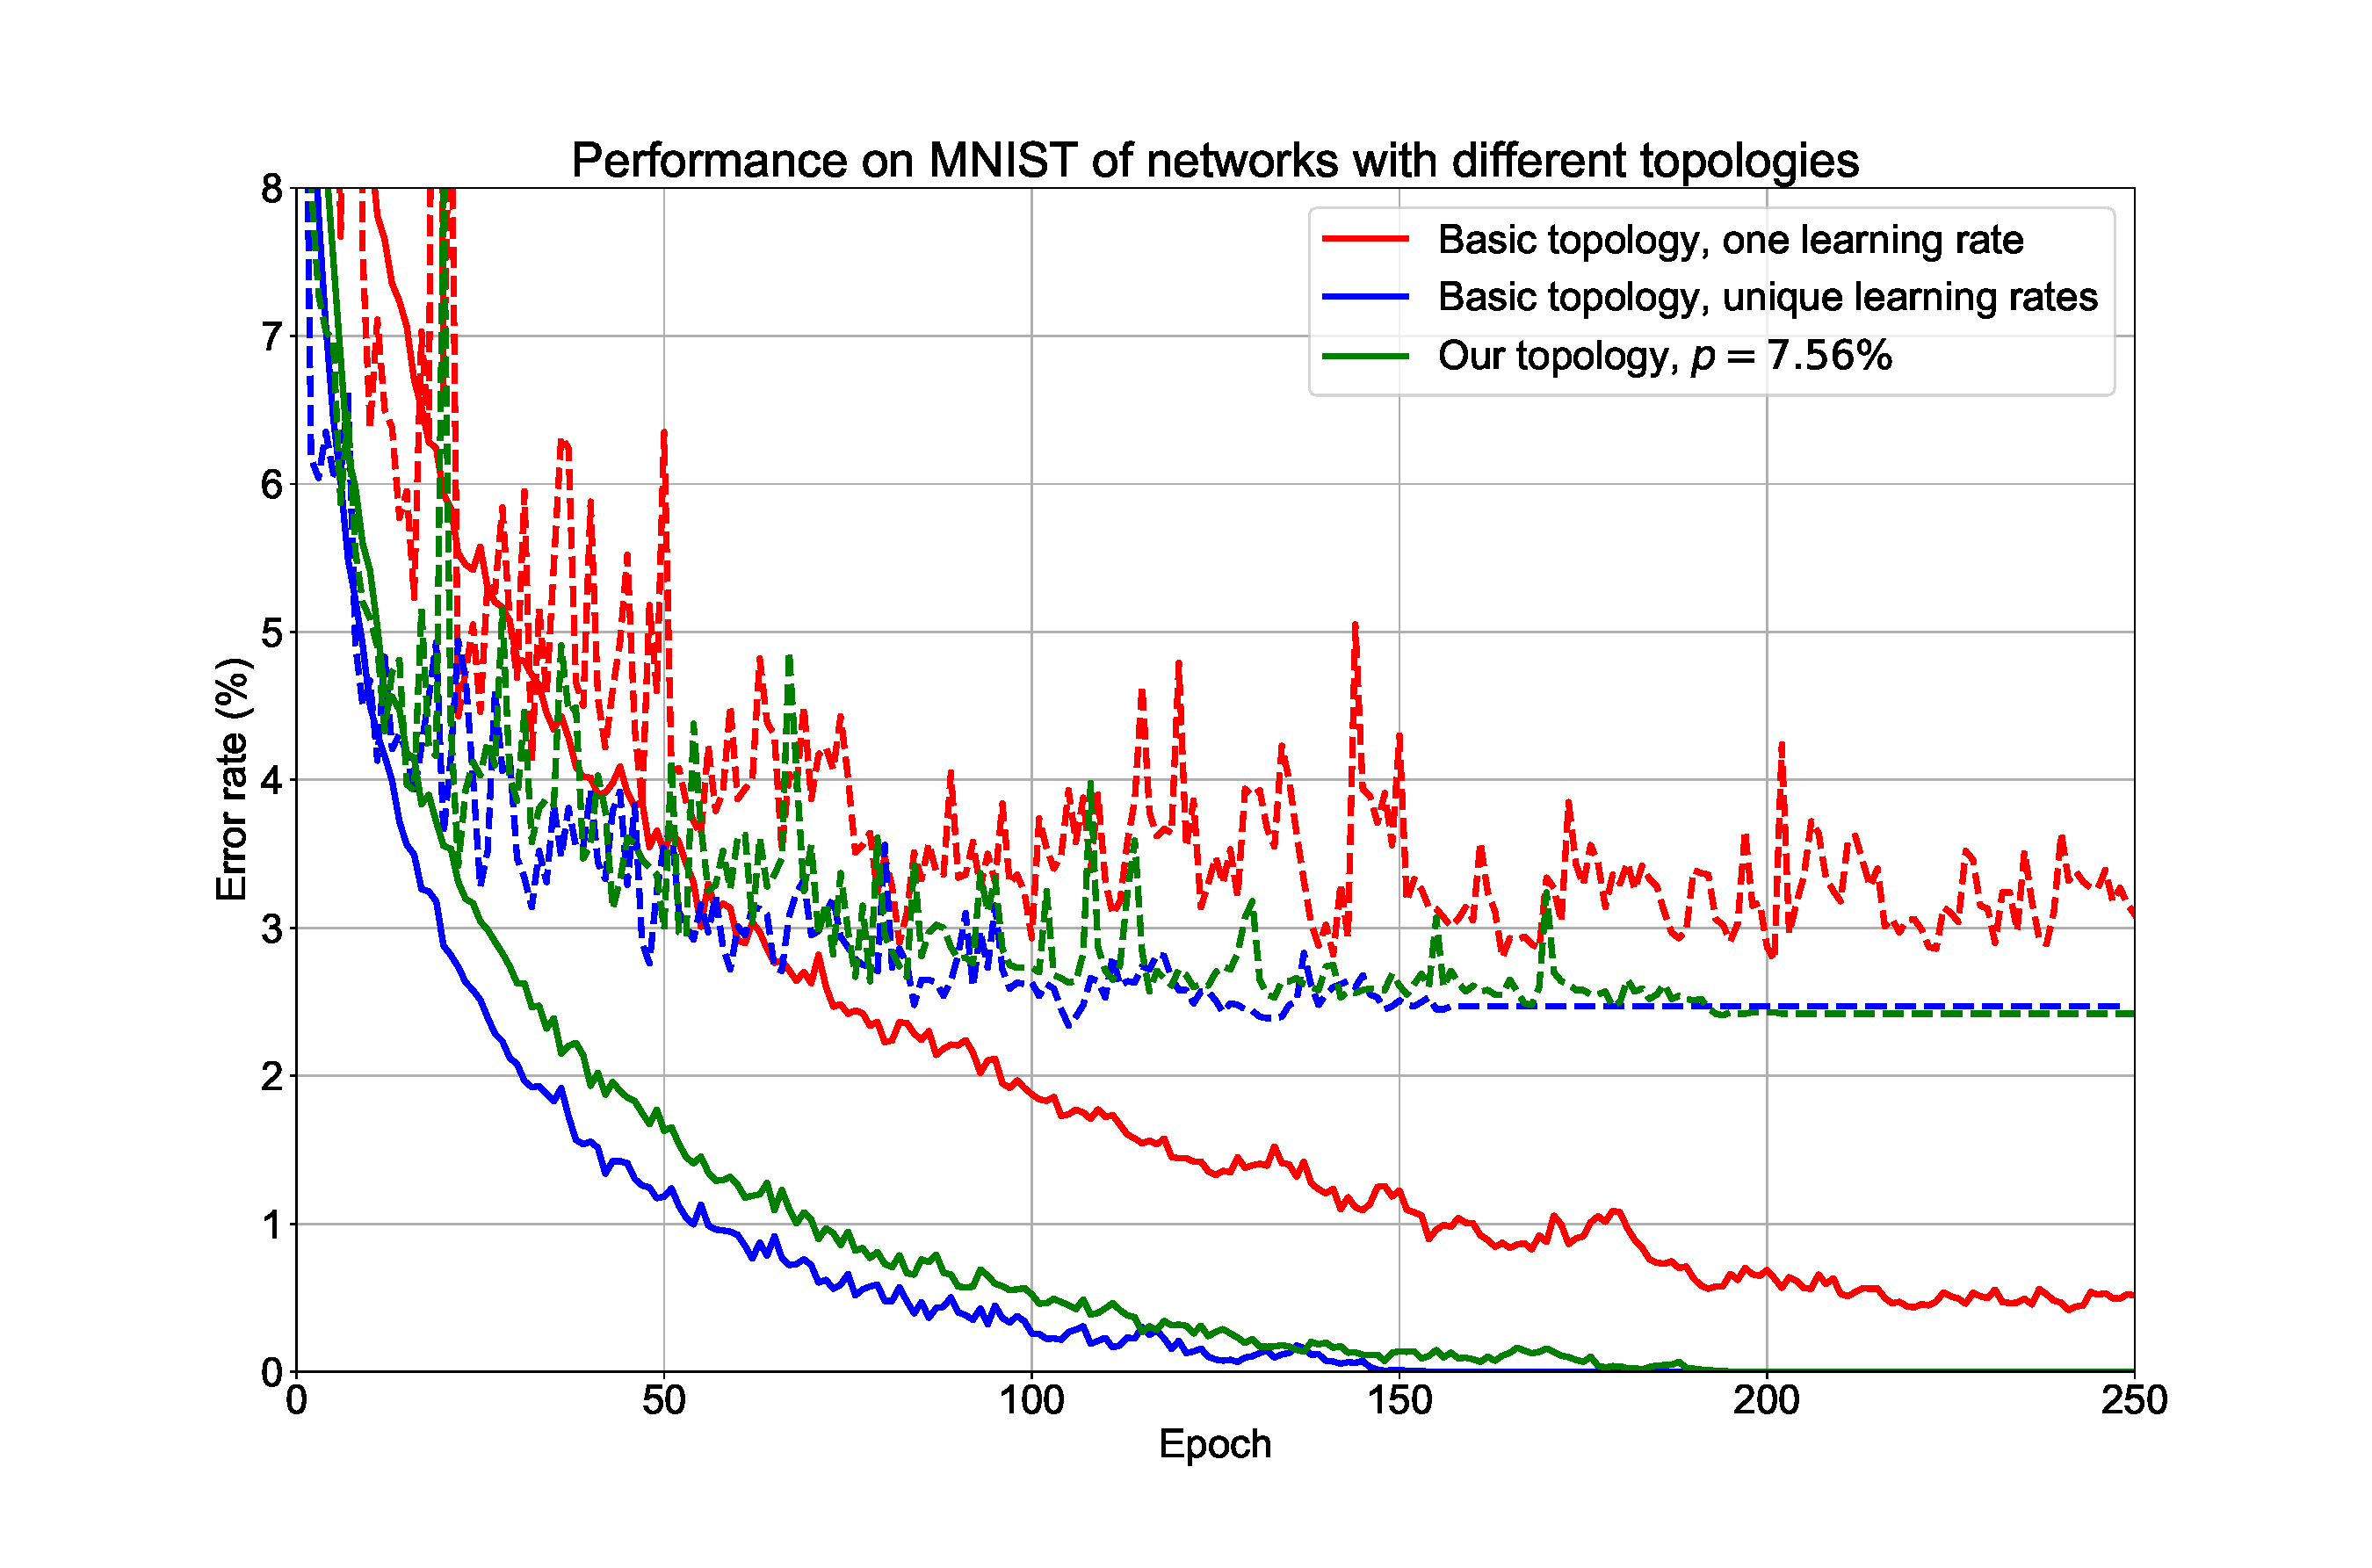
\includegraphics[width=\columnwidth]{figures/MNIST_network_comparison.pdf}
  \caption{Comparison of performance of network topologies on MNIST dataset. Dotted lines show test error and solid lines show training error. In green is a network with the layered topology and a single learning rate (section \ref{sec:basic_topology_uniform}). In orange is a network with the layered topology and unique learning rates (section \ref{sec:basic_topology}), tuned to counter the vanishing gradient problem; this is a recreation of the 5-layer network in \cite{scellier17}. In black is a network with our topology, $p=7.56\%$ (section \ref{sec:our_topology}). The network with a layered topology and a single learning rate performs poorly because it suffers from the vanishing gradient problem. The problem can be solved by introducing unique learning rates, or by implementing our topology.}
  \label{fig:mnist_comparison}
\end{figure}

We compared the three network topologies described in sections \ref{sec:basic_topology}, \ref{sec:basic_topology_uniform}, and \ref{sec:our_topology} on the MNIST dataset \cite{mnist1998}. The only hyperparameter that differed between networks was the learning rate(s); the layered network with unique learning rates used rates of .128, .032, .008, and .002 for layers from output to input, and the layered network with one learning rate and the network with our topology used a learning rate of .02. All networks used $\epsilon=.5$, $\beta=1.0$, $N_{free}=500$, $N_{weakly-clamped}=8$ and were trained for 250 epochs with 50,000 training examples, 10,000 test examples and a batch size of 20. To generate our topology we used algorithm \ref{alg:ourtop} with $p=7.56\%$ (100,000 replacements made).

\subsection{Network performance comparison}
\label{sec:network_performance}

We tracked the error rates of the three networks as they were trained and found that the network with our topology significantly outperforms the basic network with one learning rate, and achieves the same error rates as the basic network with unique learning rates after around 25\% more epochs. These results are shown in figure \ref{fig:mnist_comparison}.
\npar
 Notice that the layered network with unique learning rates converges to 0\% training error and 2.5\% test error in around 150 epochs and the network with our topology converges to 0\% training error and 2.5\% test error in around 190 epochs, whereas the layered network with one learning rate fails to converge in 250 epochs and has training and test error around .5\% higher than the other two networks. While it is possible that the basic network with one learning rate would converge given enough time, it is clearly inferior to the other two networks. It is also apparent that on the MNIST dataset, our network with a single learning rate is practically interchangeable with the layered network with unique learning rates.

\subsection{Training rates of individual pairs of layers}
\label{sec:mnist_perlayer}

\begin{figure}
  \centering
  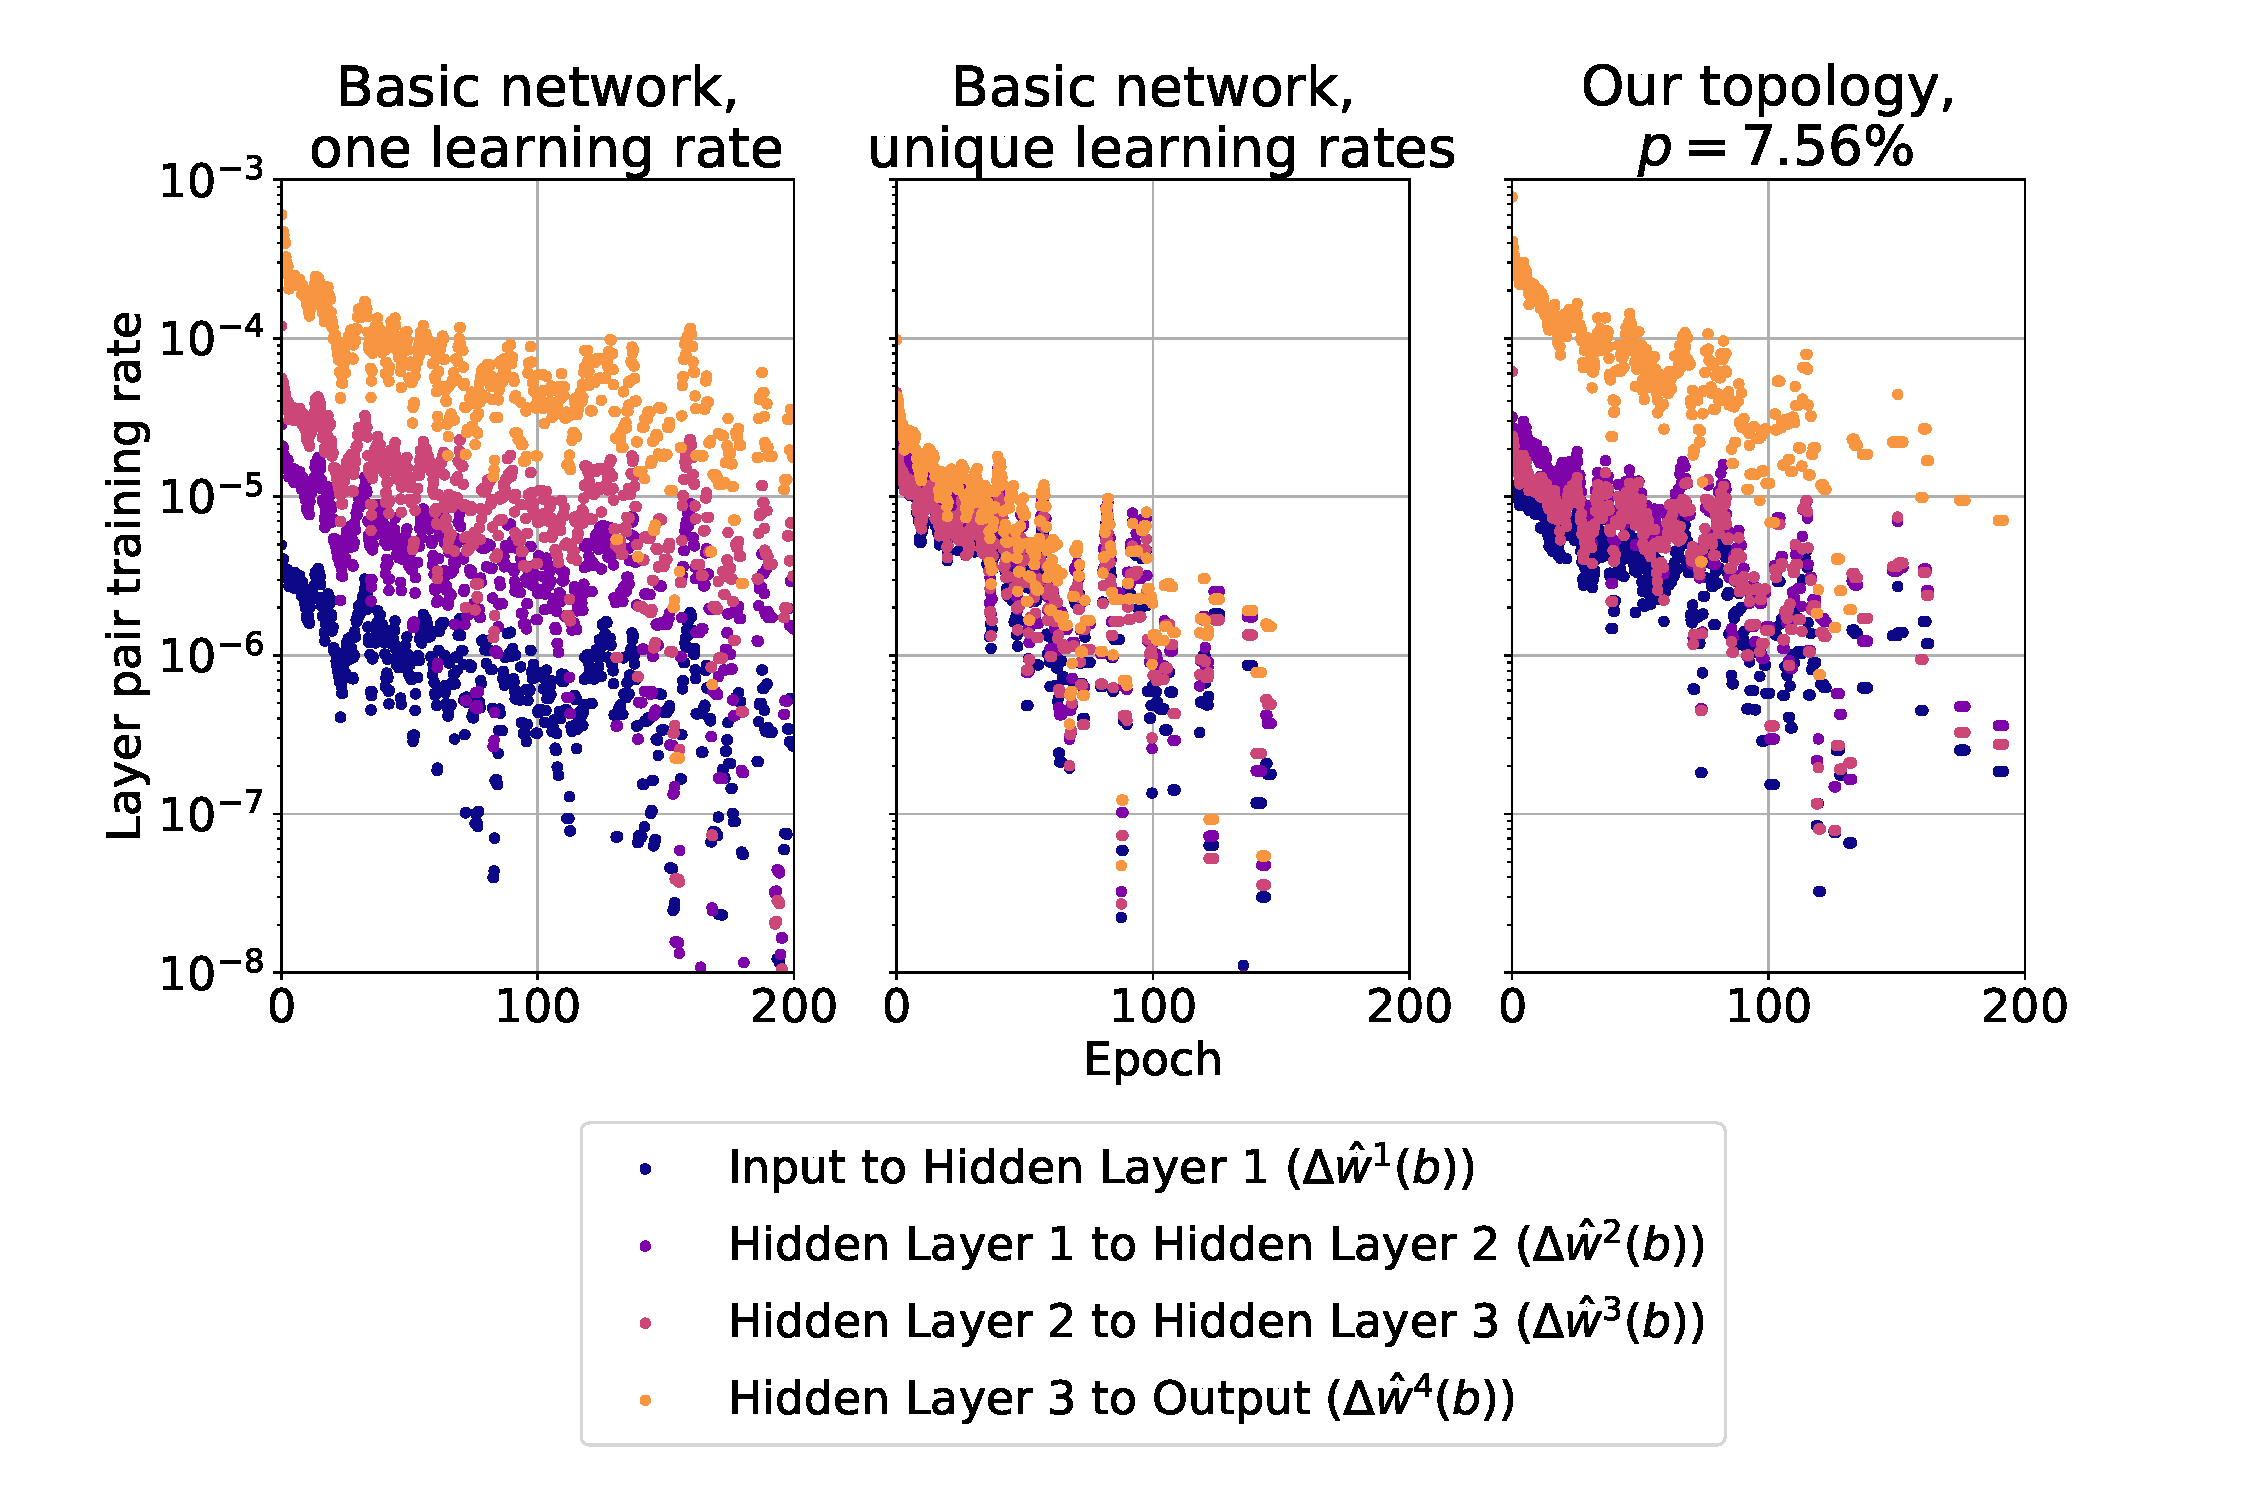
\includegraphics[width=\columnwidth]{figures/MNIST_individual_layers.pdf}
  \caption{Extent of the vanishing gradient problem in different network topologies while training on MNIST dataset. (left) A network with the layered topology and a single learning rate. The training rate of a layer decreases by a factor of $\sim 4$ with each additional layer. (center) A network with the layered topology and unique per-layer learning rates. The vanishing gradient is counteracted by hand-tuning a learning rate hyperparameter for each layer.  (right) A network with our topology, $p = 7.56\%$. The new topology eliminates the need for hand-tuning per-layer learning rate hyperparameters.}  
  \label{fig:mnist_layers}
\end{figure}

We tracked the training rates of individual pairs of layers as described in equations \ref{eqn:rms_correction} and \ref{eqn:running_avg} and found evidence that the extent of the vanishing gradient problem is the primary cause of the performance disparity seen in section \ref{sec:network_performance}. These results are shown in figure \ref{fig:mnist_layers}.
\npar
Notice that in the layered network with one learning rate there is a significant spread in the training rates of pairs of layers, with the deepest pair training at around 1\% of the rate of the shallowest pair. This problem is solved very effectively in the layered network with unique learning rates. The problem appears to be solved effectively for the deepest 3 pairs in the network with our topology, but the output layer still trains significantly faster than the deeper 3 layers. This makes sense if we assume that the important factor in a layer's training rate is its expected path length to the target layer, because every neuron in the output layer connects to the target layer through a single connection, whereas paths starting at deeper neurons must first pass through the output layer before connecting to the target layer.

\subsection{Error rate after one epoch as connections are added}
\label{sec:mnist_1epoch}

\begin{figure}
  \centering
  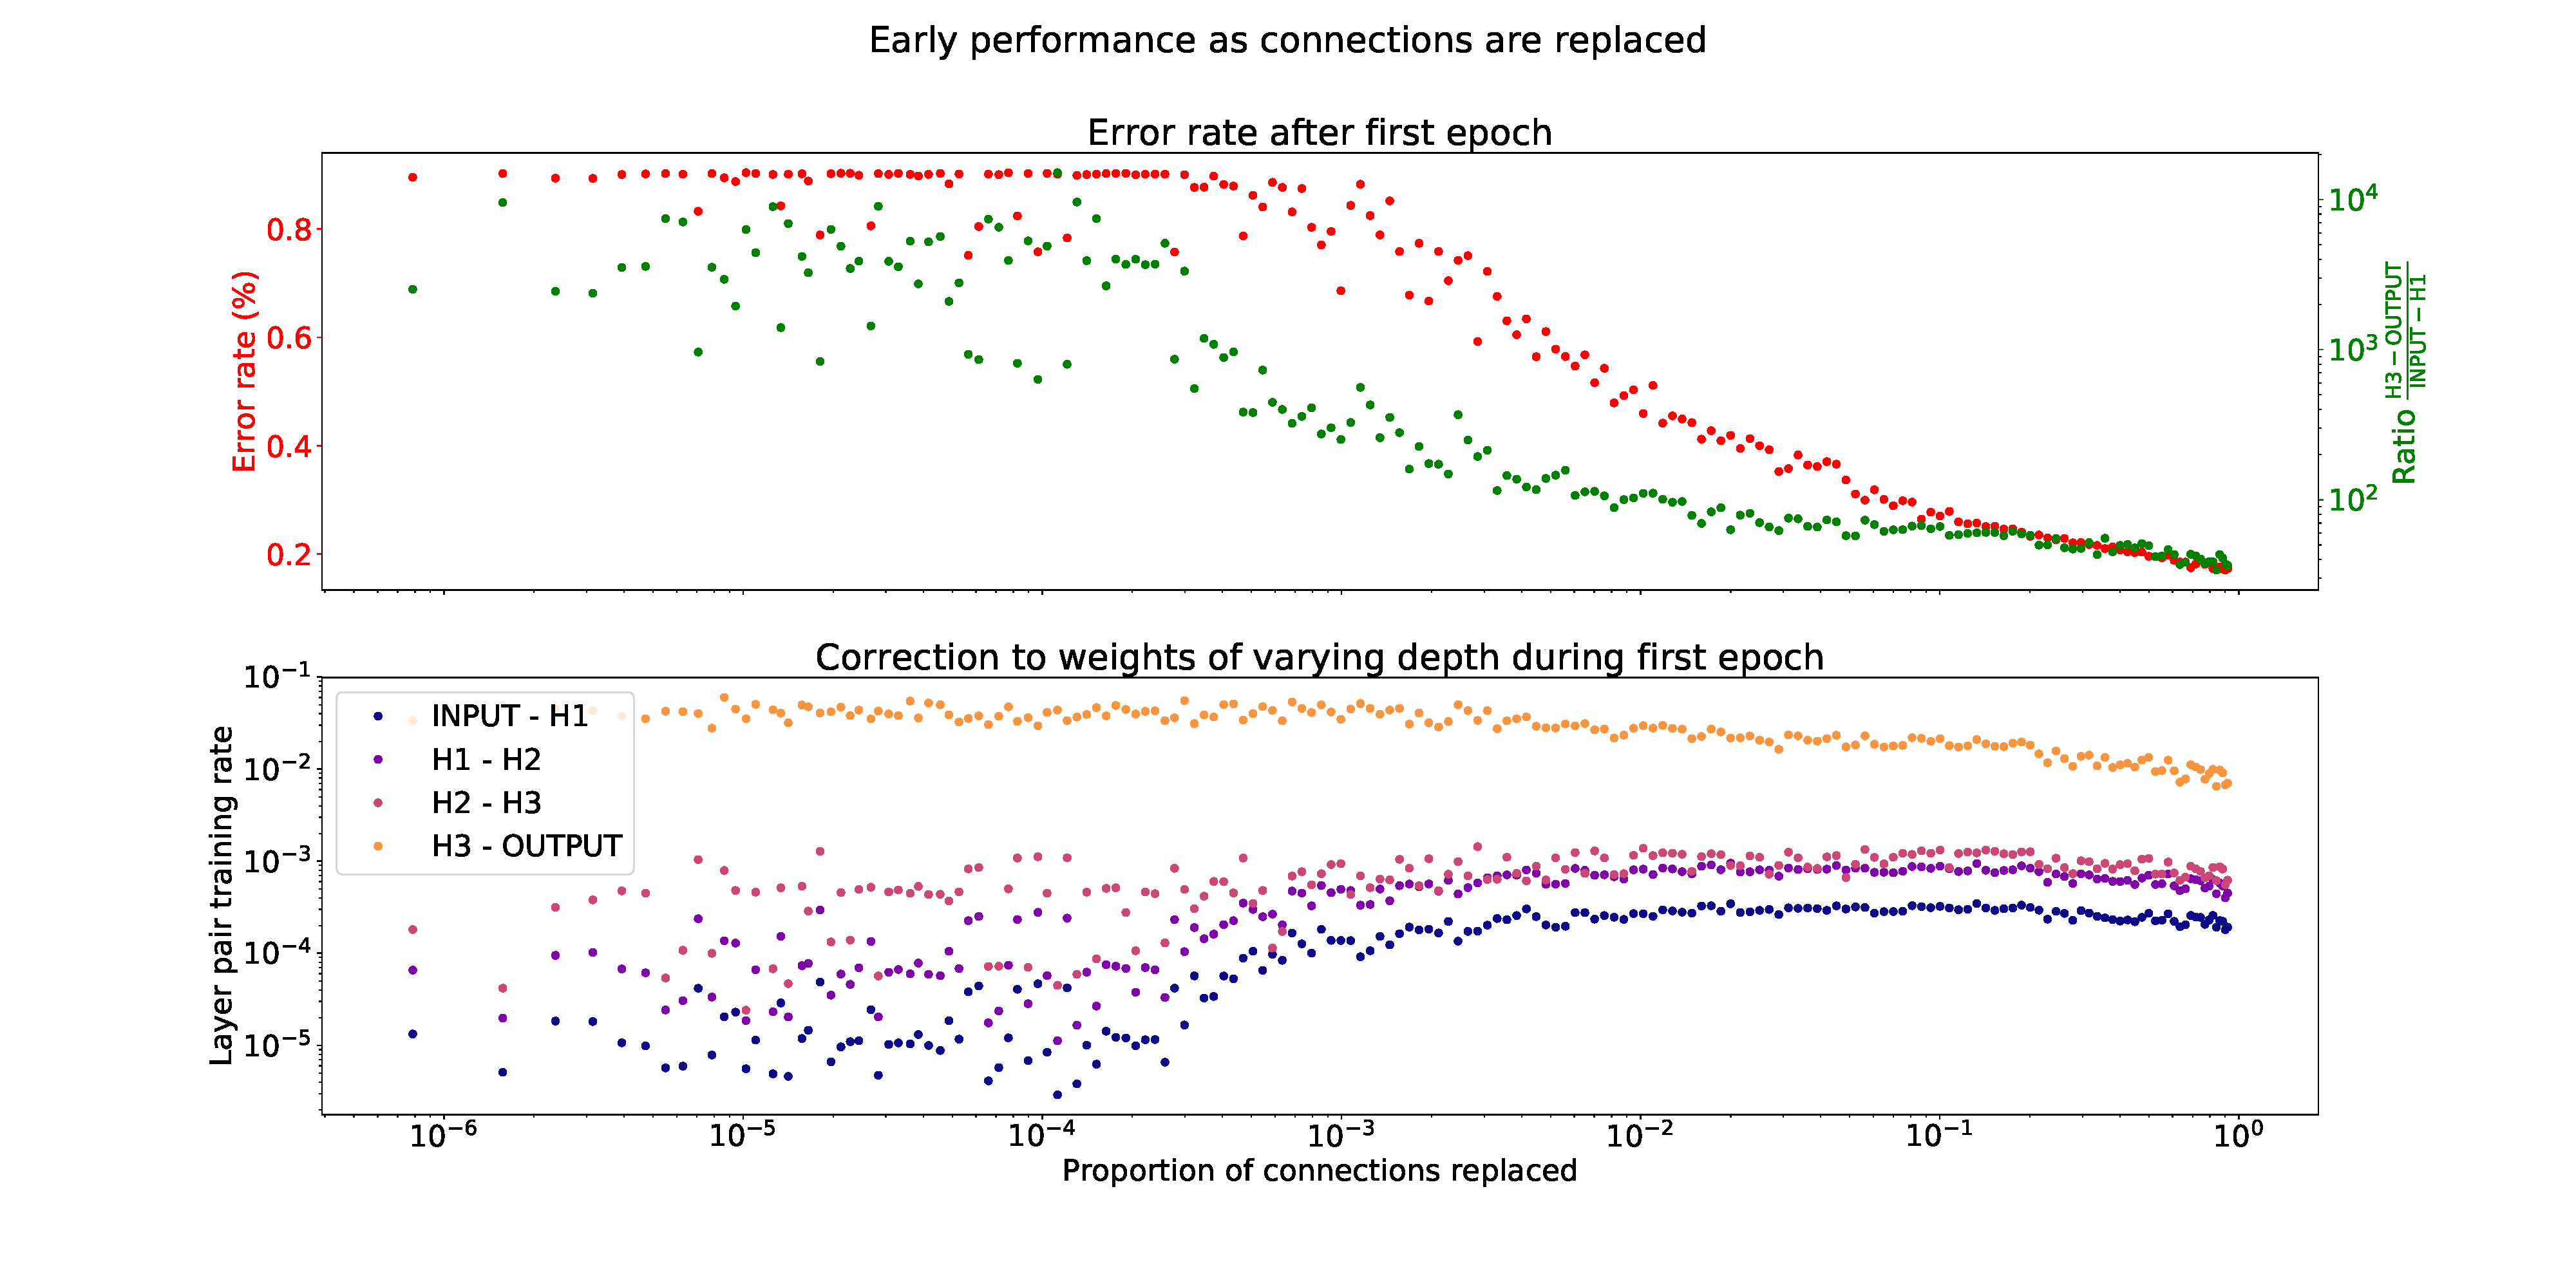
\includegraphics[width=\columnwidth]{figures/MNIST_one_epoch_performance.pdf}
  \caption{Performance of a network with  varying $p$ during the initial stages of training. (top) The training error after one epoch. (bottom) Training rate for each layer after one epoch. There is little improvement for $p<.1\%$, after which the error rate decreases at a rate that is slightly slower than exponential with $p$. Improvement begins after the training rates of non-output layers converge, and improvement beyond that point is associated with convergence between the rates of the output layer and the non-output layers.}
  \label{fig:mnist_1epoch}
\end{figure}

We tracked the training error after one epoch of a network with our topology while varying $p$; the results are shown in figure \ref{fig:mnist_1epoch}.
\npar
Three regimes are evident in the figure. For $p<.1\%$, there is little improvement in the error rate as $p$ is increased, but there is substantial improvement in the uniformity of the training rates of deep layers. When $p>.1\%$, the deep layers are very uniform, and the error rate starts decreasing with $p$ at a rate that is slightly slower than exponential; at this point there is little improvement in the uniformity of deep layers, but the rate of the shallowest layer appears to move closer to those of the deeper layers.
\npar
We found that our topology performs significantly worse than the basic topology with one learning rate when few connections are replaced. This could be due to a poor weight initialization scheme for the added intralayer connections; we have noticed anecdotally that networks appear to be less-sensitive to their weight initialization scheme as connections are replaced. We have found that networks perform poorly relative to a basic network with one learning rate until $p$ is in the ballpark of 7\%. This experiment suggests that training rate will keep improving long after that, but does not show long-term performance or test performance; we suspect that a network's generalization ability will suffer for large $p$ as it loses its regimented nature.

\section{Related work}
Much research has been done in pursuit of a biologically-plausible deep learning algorithm. References \cite{lee2015, xie2003, pineda1987} describe other algorithms that approximate the gradient of a cost function locally. Reference \cite{lillicrap2014} demonstrates that networks can train through backpropagation with randomly-initialized feedback weights between neurons; the need for symmetric connection weights is not solved by equilibrium propagation and is not biologically-plausible, so this finding could potentially be applied here as well. Reference \cite{oconnor2018} implements equilibrium propagation using spiking neurons; this type of activation function is believed to be more biologically-plausible than a hardened sigmoid function. Reference \cite{bengio2015} discusses the criteria a biologically-plausible algorithm would need to satisfy. Reference \cite{bartunov2018} surveys promising biologically-motivated algorithms and evaluates their effectiveness on hard datasets.
\npar
References \cite{shainline2019, davies2018, nahmias2013} discuss neuromorphic architecture that could potentially implement equilibrium propagation.
\npar
Layer-skipping connections have been explored in other contexts. References \cite{he2015, srivastava2015} use layer-skipping connections as a linear transformation in parallel with nonlinear layers to great effect in very-deep convolutional networks. References \cite{xiaohu2011, krishnan2019} apply small-world topology to networks trained using backpropagation.
\npar
References \cite{ioffe2015, glorot2010} effectively counter the vanishing gradient problem in the context of deep networks trained using backpropagation.

\section{Discussion and Future Research}

\subsection{Characteristics of an effective network}

Our experiments indicate that networks with our topology perform poorly relative to a layered network with a single learning rate until $p$ is in the ballpark of $8\%$. It seems likely that the training rate will continue to improve as $p$ is increased to around 70\%; however, we suspect this improvement would be at the cost of a higher test error rate, because as $p$ increases a network's topology looks less-layered and more like a sparsely-connected single-layer network. We did not observe deterioration of a network's generalization ability for $p=7.56\%$; it is possible that such deterioration is not evident when training on a dataset as simple as MNIST, but would become apparent on a more-difficult dataset such as CIFAR or ImageNet.

\subsection{Factors influencing network performance}
\label{sec:disc_factors}

Contrary to our expectations, we found that a network's performance did not track closely with any of the small-world metrics (Appendix \ref{app:sw_metrics}). Good performance was achieved when algorithm~\ref{alg:ourtop} was executed with $p\approx 8\%$, which leads to a network with small $L$ and $C$ that was therefore not small-world. In retrospect we believe these metrics to be poor predictors of network performance. One reason for this may be that the characteristic path length $L$ quantifies the shortest path between two neurons, but the total number of paths is also important because a neuron's behavior is dictated by an affine transformation of all its inputs. Similarly, it can be important for a network to retain its layered nature in order to generalize well, but the clustering coefficient $C$ does not appear to be a good metric for this - e.g. a layered network without intralayer connections has a small clustering coefficient because the neighbors of a given neuron are not connected to one-another.
\npar
There are several factors other than path length that we believe affect performance with respect to $p$, and that may disguise relationships between performance and the small-world metrics. It has been shown \cite{he2015, ioffe2015} that in deep convolutional networks, performance can be improved by using layer-skipping connections to create an identity mapping or dimension-preserving linear transformation in parallel with groups of nonlinear layers to reframe their task as learning the residual of the output of earlier layers; in our implementation layer-skipping connections form a linear transformation of earlier layers, and this fact may improve performance even though only some of the dimensions of the deeper layers are transferred. Due to the discrete approximation of the network's dynamics whereby a neuron $l$ layers from the output is not influenced by a perturbation of the output until iteration $l+1$ of the approximation, deep layers experience less evolution than shallow layers during the weakly-clamped phase; since layer-skipping connections allow deeper layers to begin evolving sooner, they probably reduce this effect. As connections are replaced, a network looks less layered and more like a sparsely-connected single-layer network, so we expect that there is a tradeoff between the rate at which a network trains and its ability to generalize. In this paper our topology did not deteriorate test error relative to the original layered network, but it is possible that a network on a harder dataset such as CIFAR or ImageNet or with a higher value of $p$ would see deterioration as its topology deviates from a layered topology.



\subsection{Directions for Future Research}

There are several directions in which future research could be taken:
\begin{itemize} 
\item Finding and mathematically-justifying a weight initialization scheme for added and replaced connections.
\item Exploring the effect of adding (instead of replacing) layer-skipping connections, training a network, then removing the connections and training further, to see if there is a lasting benefit after removal; if so, connections could be used to quickly train a network in analog hardware, then removed to reduce the network's power consumption and heat load. 
\item Exploring the effect of allowing non-output connections to be directly affected in the weakly-clamped phase of training, in effect allowing neurons outside the output layer to connect to the target layer; this would likely reduce the gap between the training rates of output and hidden layers seen in figure \ref{fig:mnist_layers}. 
\item Exploring a network's test error as $p$ is increased, especially on difficult datasets such as CIFAR or ImageNet where generalization is very important.
\end{itemize}


\bibliographystyle{plain}

The U.S. Government is authorized to reproduce and distribute reprints for governmental purposes notwithstanding any copyright annotation thereon.


\bibliography{references}

\begin{appendices}


\section{Metrics of a graph's small-worldness}
\label{app:sw_metrics}

A graph's small-worldness can be characterized by its characteristic path length $L$ and its clustering coefficient $C$ \cite{watts98}. A graph is small-world if $L$ is small relative to that of a random network with the same number of vertices and edges and $C$ is not substantially smaller than that of the random network; this situation can be quantified by a small-world coefficient $\sigma$ \cite{humphries2008}. The characteristic path length is the minimum number of edges in a path joining a pair of vertices, averaged over all pairs of vertices in the network. For a graph with $N$ vertices where $l(v_i,v_j)$ denotes the smallest number of edges needed to connect vertex $v_i$ to vertex $v_j$, 
\begin{equation}
\label{eqn:charpathlength}
L=\frac{1}{N(N-1)}\sum_{i=1}^{N}\sum_{\substack{j=1\\j\neq i}}^{N}l(v_i,v_j).
\end{equation}
The neighborhood of a vertex is the set of vertices with which it shares an edge. The clustering coefficient is the proportion of pairs of vertices in the neighborhood of a given vertex that share an edge, averaged over all vertices in the network. For a graph with $N$ vertices, if $\text{N}(v_i)$ denotes the neighborhood of vertex $v_i$ and $c(v_j,v_k)=\begin{cases}1 & v_k\in\text{N}(v_j)\\0 & \text{else}\end{cases}$,
\begin{equation}
\label{eqn:clustcoeff}
C=\frac{1}{N}\sum_{i=1}^{N}\frac{1}{|\text{N}(v_i)|}\sum_{\substack{v_j\in \text{N}(v_i)\\v_k\in\text{N}(v_i)\\j\neq k}}c(v_j,v_k)
\end{equation}
The small-worldness of a graph can be quantified by a small-world coefficient
\begin{equation}
\sigma=\frac{C/C_r}{L/L_r}
\end{equation}
where $C_r$ and $L_r$ are the expected clustering coefficient and characteristic path length of a random graph with the same number of vertices and edges as the graph under consideration.


\end{appendices}



\end{document}




